\chapter{Experimental setup}
%% This chapter describes the present experimental setup.
%% The present experiment was carried out at the K1.8BR beamline of the Hadron Facility at J-PARC.
%% First, a brief description of J-PARC is given, followed by a description of the Hadron Facility and the slow beam extraction there.
%% Next, the secondary beam transport and particle selection methods are described, including the electromagnet setup used for them.

%% Then, detectors in the experimental area are described.
%% These detectors consist of three main parts.
%% One is the beamline detector system for analysing the beam,
%% the second is the forward detector system for analysing the forward scattered nucleons
%% and the third is the cylindrical detector system (CDS) for measuring the particles that decay from the produced hyperons.
%% In addition, the trigger circuit and the DAQ system are described, which digitize the detector signals and import into a PC.

%% \section{Experimental facility}
\subsection{J-PARC}

The J-PARC is located at the Tokai village in Ibaraki Prefecture.
J-PARC, which means Japan Proton Accelerator Research Complex, consists of some facilities,
which are nuclear transmutation facility, materials, and the Material Life Science Experimental Facility, Neutrino Experimental Facility, and Hadron Experimental Facility\cite{JPARC_had}.
The concept of the J-PARC is to provide various secondary beam for the above purpose.
The J-PARC has three accelerators,
first one is linac which is injector and accelerates proton beam to $400$MeV$/c$,
second is RCS (Rapid Cycling Synchrotrons) which accelerates proton beam to $3$GeV, which was provided to materials and life experimental facility and muon facility.
Next is MR (Main Ring) which accelerates proton beam to $30$GeV$/c$, which beam was extracted by two methods.
One is the fast extraction (FX) for the Neutrino Experimental Facility to produce a neutrino beam which transported to the super Kamiokande.
The other is the slow extraction (SX) for the Hadron Experimental Facility.
In this extraction, banched beam in the MR is gradually extracted as scraping.
For this purpose, the $30$GeV$/c$ proton beam was extracted about 2-second with a 5.2-second repetition cycle in the present experimental.

This continuous beam is irradiated on the primary target that is 6mm $\times$ 6mm $\times$ 66mm golden block
to generate secondary beam which includes anti-proton, pion, kaon and so on that is not naturally exist.
The secondary beam is transported to several beamlines.

The present experiment ix performed at the K1.8BR beamline, which was placed at north of the hadron facility and branced from the K1.8 beamline
which is optimized for beam whose momentum is around $1.8$GeV$/c$.

%% \subsection{K1.8BR beam line}
The K1.8BR beamline was planned to use low momentum kaon beam whose upper limit is 1.2 $GeV/c$.
Such kaon decays with short decay time, so beam line length should be short.
So, our beamline length was designed at about 31m by branching the K1.8 beamline.
Fig \ref{fig:K18BR} shows a schematic view of the K1.8BR beamline.

The D1 magnet accumulates secondary particles with the 6-degree aperture and the D2 magnet selects a specific momentum beam with $\pm$ 3\% momentum bite.
% From the D1 magnet to the D2 magnet accumulated secondary beam and selected specific momentum.
Intermediate focus slit (IF Slit) defined beam profile to increase the number of kaon beam while keeping good kaon and another particle ratio.
Kaon and other particles were separated by the electrostatic separator (ES1) using vertical direction statical electronic field
which uses the principle that different mass charged particles pass different trajectories by the electrical field.
The kaon beam was kicked up by the CM1 magnet, was bent in the opposite direction by ES1 and was kicked to parallel direction by the CM2 magnet.
Other particles pass through different position of vertical direction at mass slit1 (MS1), so these were intercepted by the MS1.
% Other particles pass through different virtical position at mass slit1 (MS1) which was intercepted by the MC1,
Also, the horizontal directional slit of the MS1 defines the dispersive of the beam.
The D3 magnet switched beam to the K1.8 or the K1.8BR.
After the D3 magnet, an SQDQD system is employed to focus the beam on the experimental target at FF of the K1.8BR beam line.
The first-order beam envelope calculated by the TRANSPORT code \cite{TRANSPORT} is shown in Fig \ref{fig:TRANSPORT}.

The data for the $d(K^-, p)$ has been taken in May-June in 2016 which is so-called as MR-RUN69 and the data for the $d(K^-, n)$ has been taken in Jan-Feb in 2018 which is so-called as MR-RUN78.

\begin{table}
  \caption[Parameters of the beam-line magnets.]{Parameters of the beam-line magnets. D5 field is a typical monitored value. Other field values are interpolations of measured points.}
  \centering
  \hspace{1cm}
  \begin{tabular}{llccccc}
    \hline\hline
    Element &       J-PARC  &       Gap or  &       Effective       &       Bend    &       Current &       Field at pole   \\
    &       designation     &        bore/2 (cm)    &       length (cm)     &       (deg)   &       (A)     &       (kG)    \\
    \hline
    D1      &       5C216SMIC       &       8       &       90.05   &       10      &       -369    &       -6.7444    \\
    Q1      &       NQ312MIC        &       8       &       67.84   &               &       -357    &       -3.075  \\
    Q2      &       Q416MIC &       10      &       87.04           &               &       -668    &       3.872   \\
    D2      &       8D218SMIC       &       15      &       99.65   &       15      &       -698    &       -8.7673 \\
    \hline
    IF-H    &       \multicolumn{4}{l}{Movable horizontal slit for acceptance control}              &               &               \\
    IF-V    &       \multicolumn{4}{l}{Movable vertical slit, (y$|\phi$)=0}                                 &               &               \\
    \hline
    Q3      &       Q410    &       10      &       54.72   &               &       -679    &       -4.108  \\
    O1      &       O503    &       12.5    &       15      &               &       -15     &       -0.29   \\
    Q4      &       Q410    &       10      &       54.72   &               &       -776    &       4.692   \\
    S1      &       SX504   &       12.5    &       27.6    &               &       -42     &       -0.29   \\
    CM1     &       4D604V  &       10      &       20      &       (0.856) &       348     &       1.633   \\
    ES1     &       Separator  &    10      &       600     &               &       \multicolumn{2}{c}{E=-500 kV/10 cm}     \\
    CM2     &       4D604V  &       10      &       20      &       (0.856) &       348     &       1.630   \\
    S2      &       SX504   &       12.5    &       27.6    &               &       -136    &       1.02    \\
    Q5      &       NQ510   &       12.5    &       56      &               &       -498    &       4.218   \\
    Q6      &       NQ610   &       15      &       57.2    &               &       -535    &       -4.316  \\
    \hline
    MOM     &       \multicolumn{5}{l}{Movable horizontal slit for momentum acceptance control}             &               \\
    MS1     &       \multicolumn{4}{l}{Movable vertical slit for $K$-$\pi$ separation }                                     &               &               \\
    &       \multicolumn{4}{l}{($y|\phi$)=0, ($y|y$)=0.844, ($y|\theta\phi$)=($y|\phi\delta$)=0}            &               &               \\
    \hline
    D3      &       6D330S  &       15      &       165.1   &       20      &       210     &       -7.064  \\
    S3      &       SX404   &       10      &       20      &               &       -34     &       -1.062  \\
    Q7      &       Q306    &       7.5     &       30.34   &               &       -464    &       4.026   \\
    D4      &       8D440S  &       20      &       198.9   &       60      &       -1938   &       -17.906 \\
    Q8      &       NQ408   &       10      &       46.5    &               &       -110    &       0.671   \\
    D5      &       8D240S  &       20      &       195.9   &       55      &       -1666   &       -16.437 \\
    \hline\hline
  \end{tabular}
  \label{tab:BL_magnet}
\end{table}

\begin{table}[htbp]
  \centering
  \begin{tabular}{ll}
    \hline \hline
    Primary beam momentum       & 30 GeV/c proton      \\
    Primary beam power          & 50kW \\
    Proton per spill            & $4.8 \times 10^{13}$ \\
    Repetition cycle            & 5.2 sec \\
    Spill Length                & 2 sec \\
    Spill suty factor           & 50\%  \\
    Spill extraction efficiency & 99.5 \% \\
    \hline
    Production target & Au(50~\% loss)\\
    Production angle  & 6 degrees \\
    Length (T1-FF)    & 31.3 m \\
    Momentum range    & 1.2 GeV/c max. \\
    Acceptance        & 2.0 msr$\cdot$\% ($\Delta\Omega\cdot\Delta p/p$)\\
    Momentum bite     & $\pm$ 3 \% \\
    \hline
  \end{tabular}
  \caption{
    Parameters of the K1.8BR beamline and typical operation condition
  }
  \label{tab:K18BR}
\end{table}


\begin{figure}[htbp]
  \centering
  \includegraphics[width=8cm]{pic/experiment/K18BR.eps}
  \caption{
    Schematic view of the K1.8BR beam line.
  }
  \label{fig:K18BR}
\end{figure}

\begin{figure}[htbp]
  \begin{centering}
    \includegraphics[width=8cm]{pic/experiment/optics.eps}
    \caption{
      First-order beam envelope calculated by the TRANSPORT.
    }
    \label{fig:TRANSPORT}
  \end{centering}
\end{figure}



%% \section{Beamline}

\subsection{BHD and T0}
The beam particles are kaon is confirmed by the TOF method using beamline hodoscope detector (BHD) and time-zero counter (T0) in the offline analysis.
The T0 is located immediately downstream of the AC.
The BHD is located between the D5 and D4 magnets, approximately 7.7m upstream of T0, i.e. the flight length is 7.7m.

The T0 is a 5-segment plastic scintillation counter array 160mm (high) $\times$ 32mm (width) $\times$ 10mm (thick), with an effective area of 160mm $\times$ 160mm.
The T0 is installed rotated 45 degrees with respect to the beam direction as the beam is horizontally spread at the T0.
A counter uses the Saint-Gobain BC420 scintillator and attached readout which is 3/4 inch Hamamatsu H6612B photomultipliers to both sides of the scintillator.

The BHD is a 20-segment plastic scintillation counter array 160mm (high) $\times$ 20mm (width) $\times$ 5mm (thick), with an effective area of 200mm (horizontal) $\times$ 160mm (vertical).
A counter uses the same photomultipliers as the T0 counter.
The BHD is installed at the most upstream of the beamline and the number of beams per spill is a few M ($\times 10^6$)events,
so the photomultipliers are attached high voltage booster to the last three dynodes to avoid gain drop due to high current by high rate beam.

\subsection{Beam line chamger}
\begin{figure}[htbp]
  \centering
  \begin{tabular}{ccc}
    \begin{minipage}{0.33\hsize}
      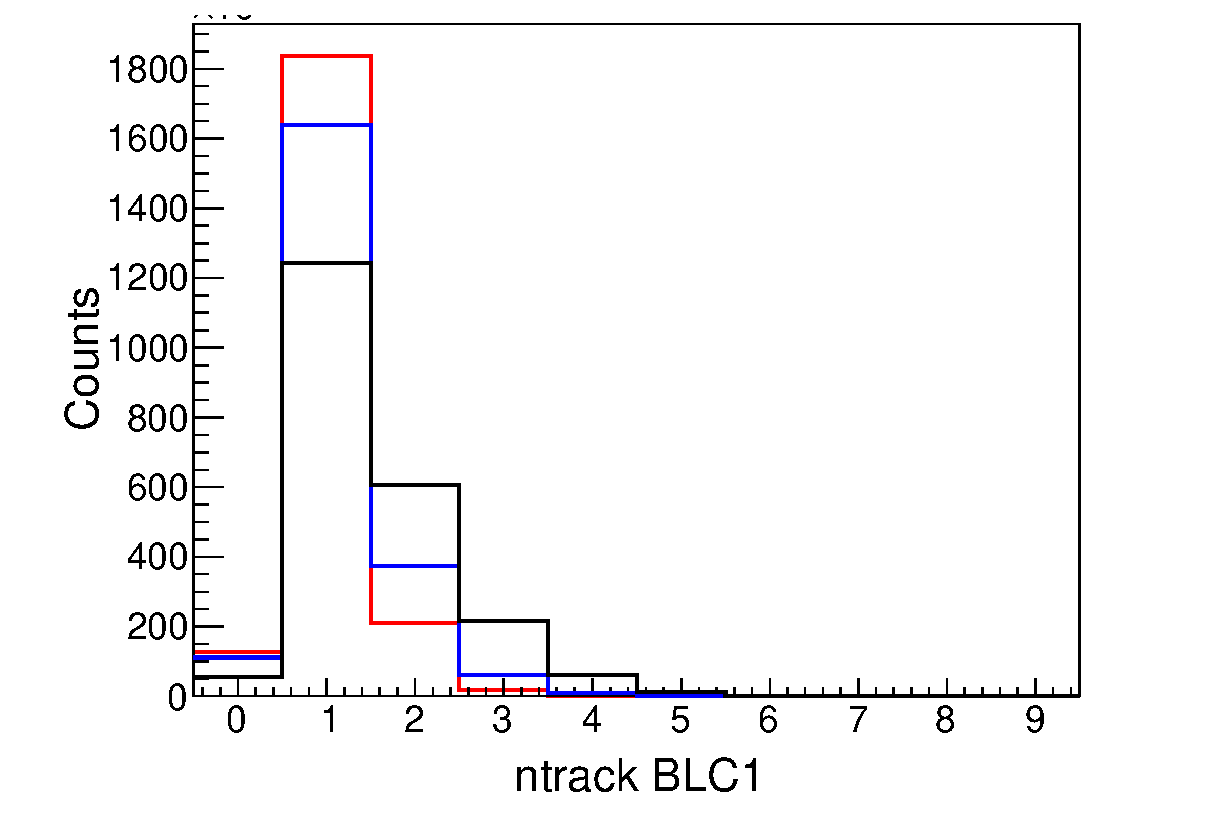
\includegraphics[width=4cm]{../pic/Run78/BL/nBLC1.eps}
    \end{minipage}
    \begin{minipage}{0.33\hsize}
      \includegraphics[width=4cm]{../pic/Run78/BL/BLC1_time.eps}
    \end{minipage}
    \begin{minipage}{0.33\hsize}
      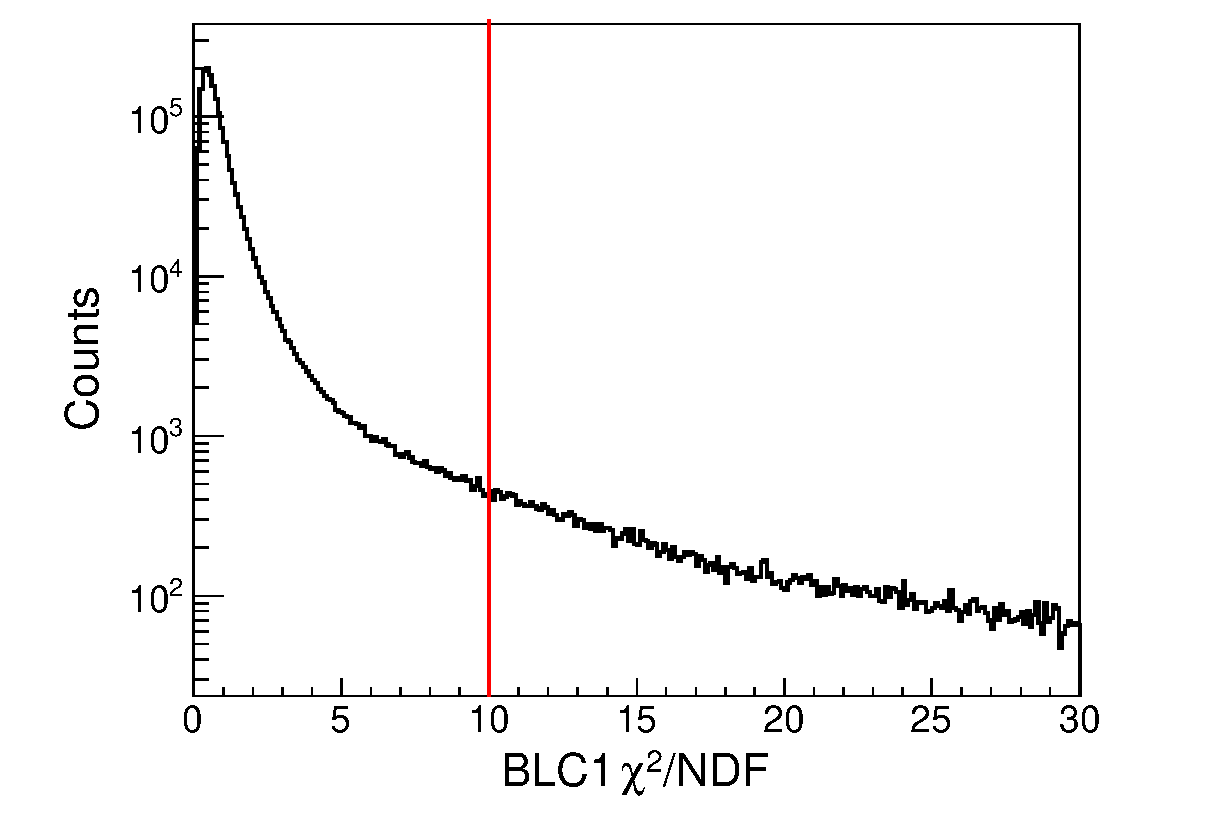
\includegraphics[width=4cm]{../pic/Run78/BL/BLC1_chi2.eps}
    \end{minipage}
  \end{tabular}
  
  \begin{tabular}{ccc}
    \begin{minipage}{0.33\hsize}
      \includegraphics[width=4cm]{../pic/Run78/BL/nBLC2.eps}
    \end{minipage}
    \begin{minipage}{0.33\hsize}
      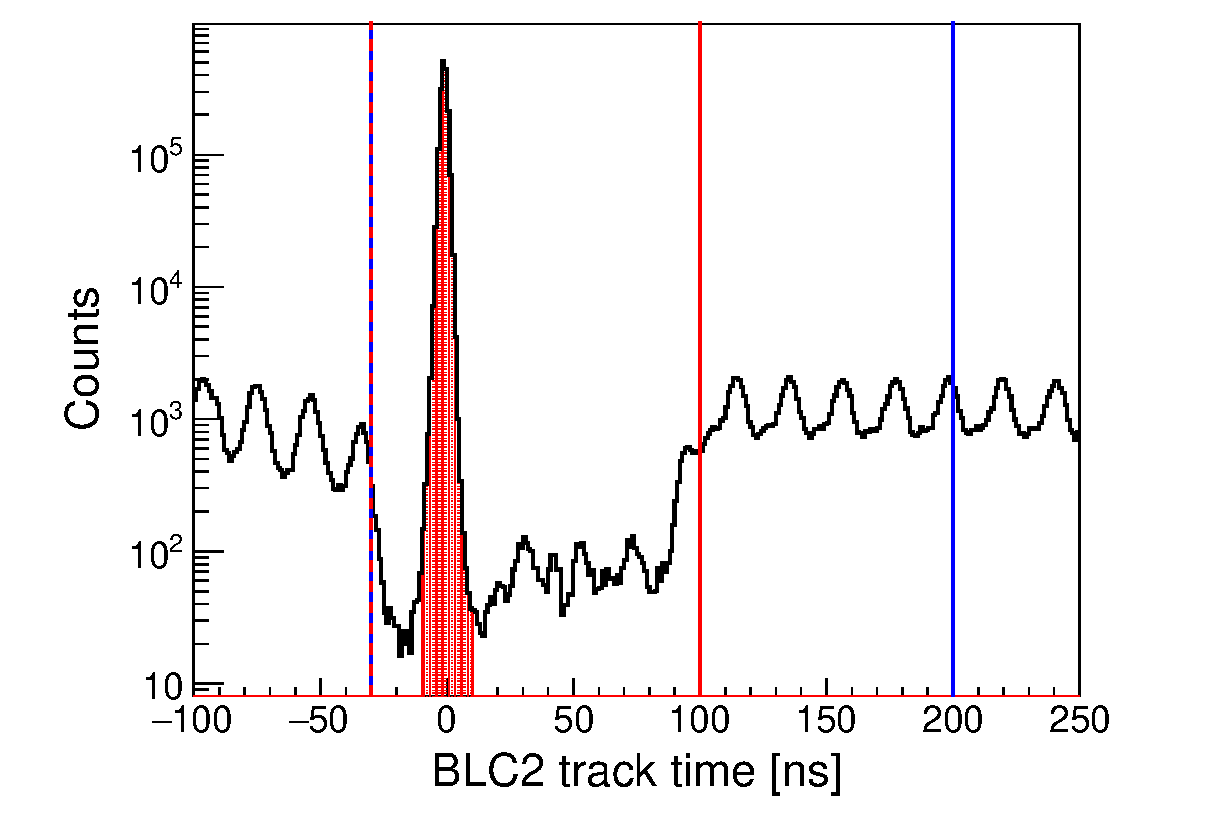
\includegraphics[width=4cm]{../pic/Run78/BL/BLC2_time.eps}
    \end{minipage}
    \begin{minipage}{0.33\hsize}
      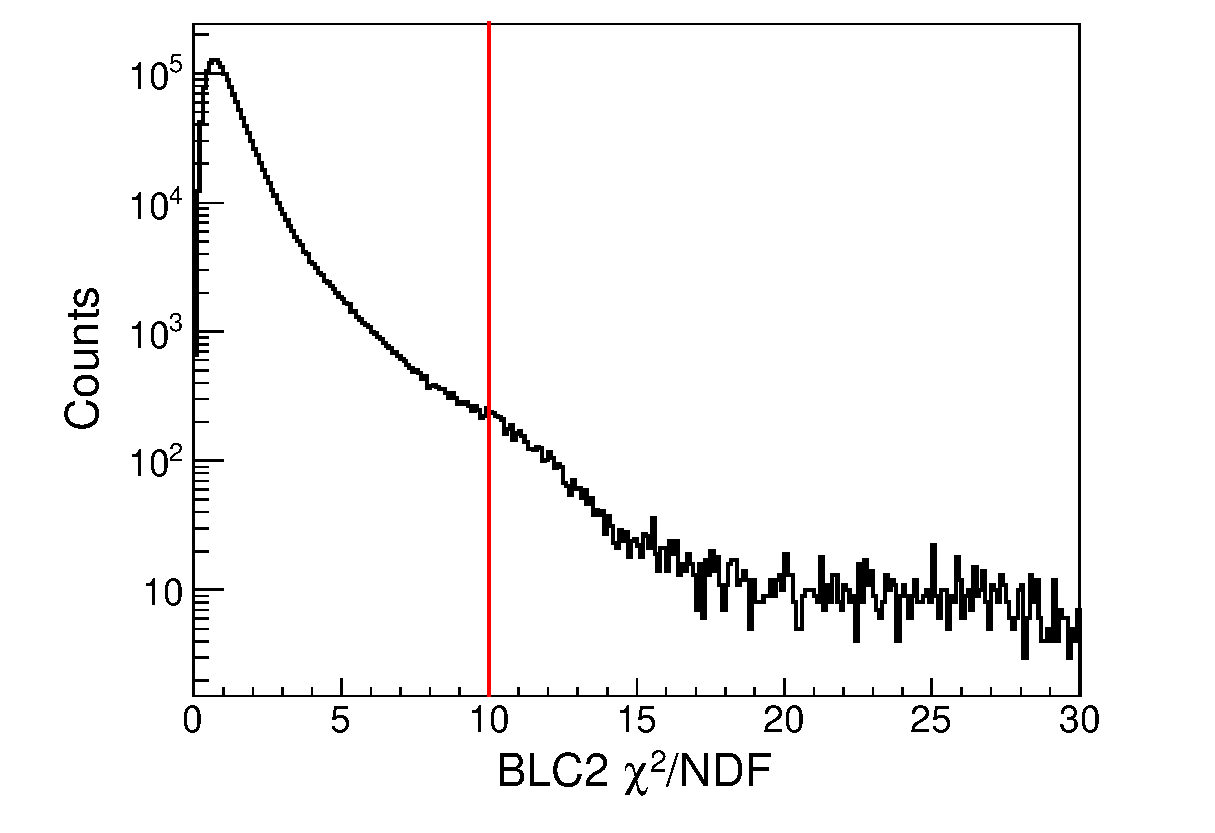
\includegraphics[width=4cm]{../pic/Run78/BL/BLC2_chi2.eps}
    \end{minipage}
  \end{tabular}
  
  \begin{tabular}{ccc}
    \begin{minipage}{0.33\hsize}
      \includegraphics[width=4cm]{../pic/Run78/BL/nBPC.eps}
    \end{minipage}
    \begin{minipage}{0.33\hsize}
      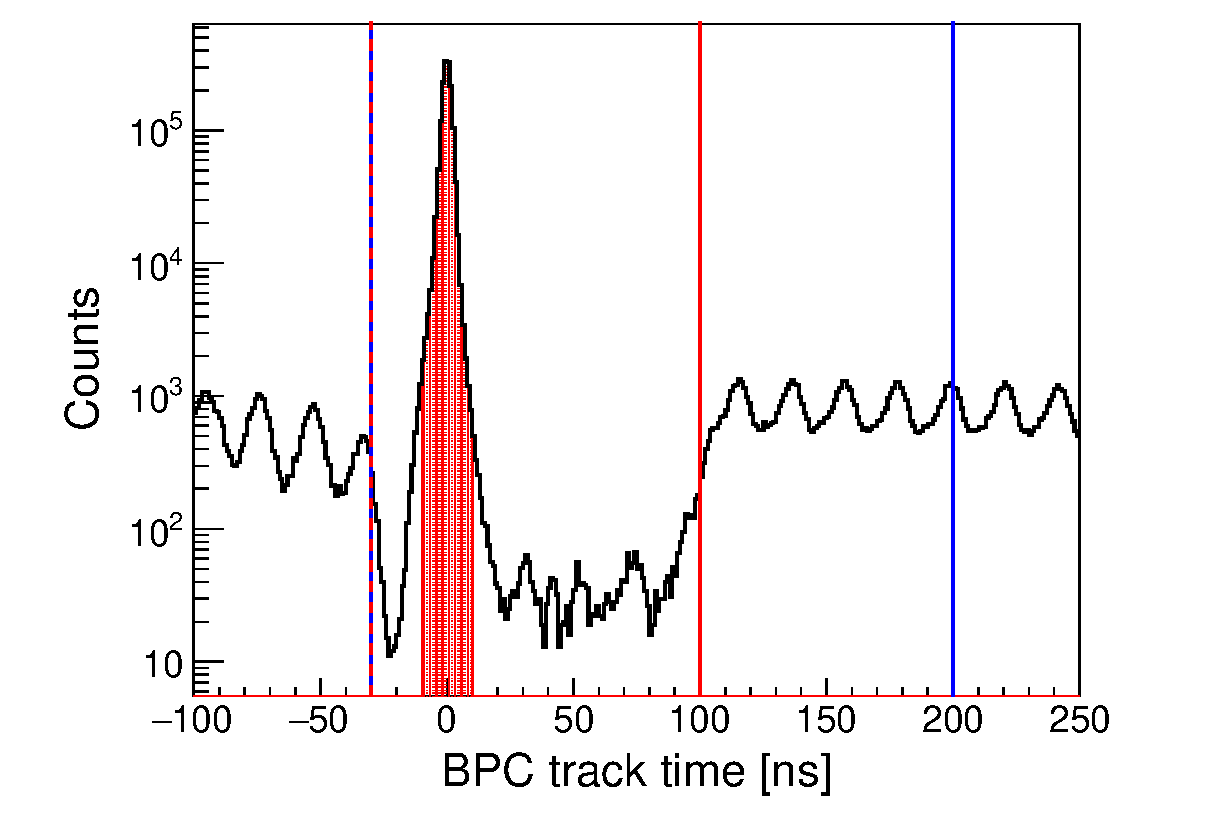
\includegraphics[width=4cm]{../pic/Run78/BL/BPC_time.eps}
    \end{minipage}
    \begin{minipage}{0.33\hsize}
      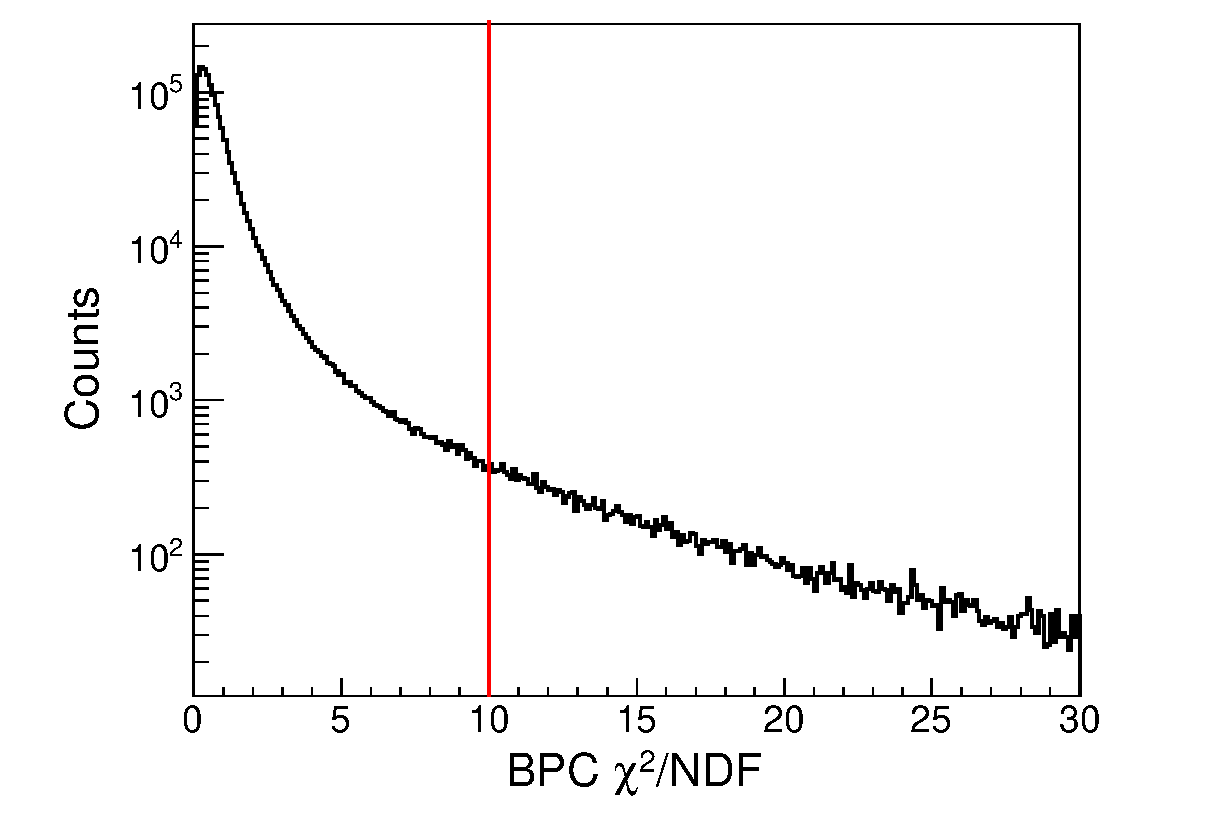
\includegraphics[width=4cm]{../pic/Run78/BL/BPC_chi2.eps}
    \end{minipage}
  \end{tabular}
  \caption{
    The left, the middle and the right figures show the number of tracks, track time and $\chi/NDF$, respectively.
    Color plots in the left figure indicate some time window.
    % Black, blue, red indicate all, $-30\sim200$[ns], $-30\sim100$[ns], respectively.
    The above, the middle and the down figures represent BLC1, BLC2 and BPC, respectively.
    The BPC was described after.
  }
  \label{fig:BLC_etc}
\end{figure}
BLC1 and BLC2 were installed upstream and downstream of the D5 magnet, respectively to measure beam momentum using the transfer matrix of the D5 magnet.
These are planer the type drift chamber whose drift length was calculated using the X-T map, which was the integration of drift time.
The track time of BLC was estimated from timing signals of pair plane due to constant drift length.
SX beam has RF-structure seems like the center figures of Fig\ref{fig:BLC_etc}, so we select synchronization about beam which indicates the red hatched region.
The left figures represent the number of tracks, in which black, blue, and red indicate time window of all, $-30\sim100$[ns], and $-30\sim200$[ns], respectively.
We select 1track events in red time window selection to keep statistics.
The right figures show $\chi^2/NDF$ distribution after 1track selection.
We accepted $\chi^2/NDF<10$ events as good track.




%% \section{Target system} \label{sec:target}
\subsection{Luquid $D_2$ target system}

\begin{figure}[htbp]
  \centering
  \includegraphics[width=10cm]{pic/experiment/d2-cryo.eps}
  \caption{
    Schematic drawing of the liquid $D_2$ cryostat.
  }
  \label{fig:d2_cryo}
\end{figure}


A side view of the cryostat for the liquid $D_2$ target is shown in Fig\ref{fig:d2_cryo}.
Deuterium is stored 1000$l$ in a tank as gases which is room temperature and 2atm keeping positive pressure after liquefaction for avoiding contamination from other materials.
The $D_2$ gas is fed into the cryostat through the top flange.
Cooling of $D_2$ is performed by the Gifford–McMahon (G–M) refrigerator (Sumitomo Heavy Industries, Ltd., RDK-145D and CSA-71A) built into the cryostat.
The cooling is performed by 2-step.
The cooling power at the first and second stages is 35$W$ at 50K and 1.5$W$ at 4.2K, respectively.
A copper plate is anchored to the first-stage cold head of the G-M refrigerator in inlet pipe for the pre-cooling of the $D_2$.
Another inlet pipe is directly connected through the top flange to the head exchanger for measuring the pressure of the $D_2$ target inside of the heat exchanger.
Since this pipe has a larger conductance, a safety valve that prevents a sudden pressure rise is also connected to it.
The $D_2$ gas is cooled in the heat exchanger where the second stage of the G–M refrigerator is thermally contacted.

\begin{figure}[htbp]
  \begin{tabular}{cc}
    \begin{minipage}{0.7\hsize}
      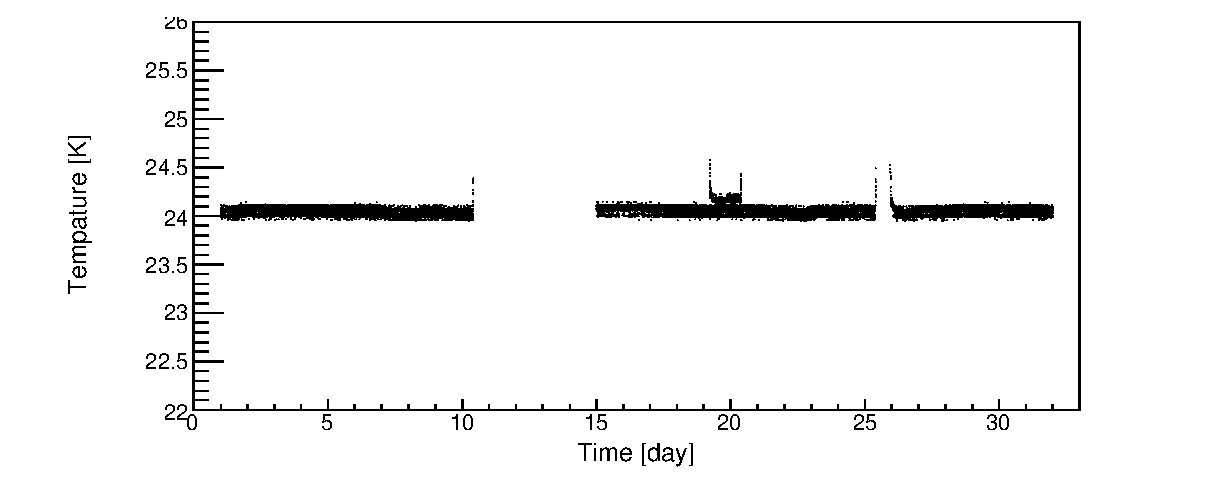
\includegraphics[width=8cm]{../pic/Dron/target/target_temp.eps}
    \end{minipage}
    \begin{minipage}{0.3\hsize}
      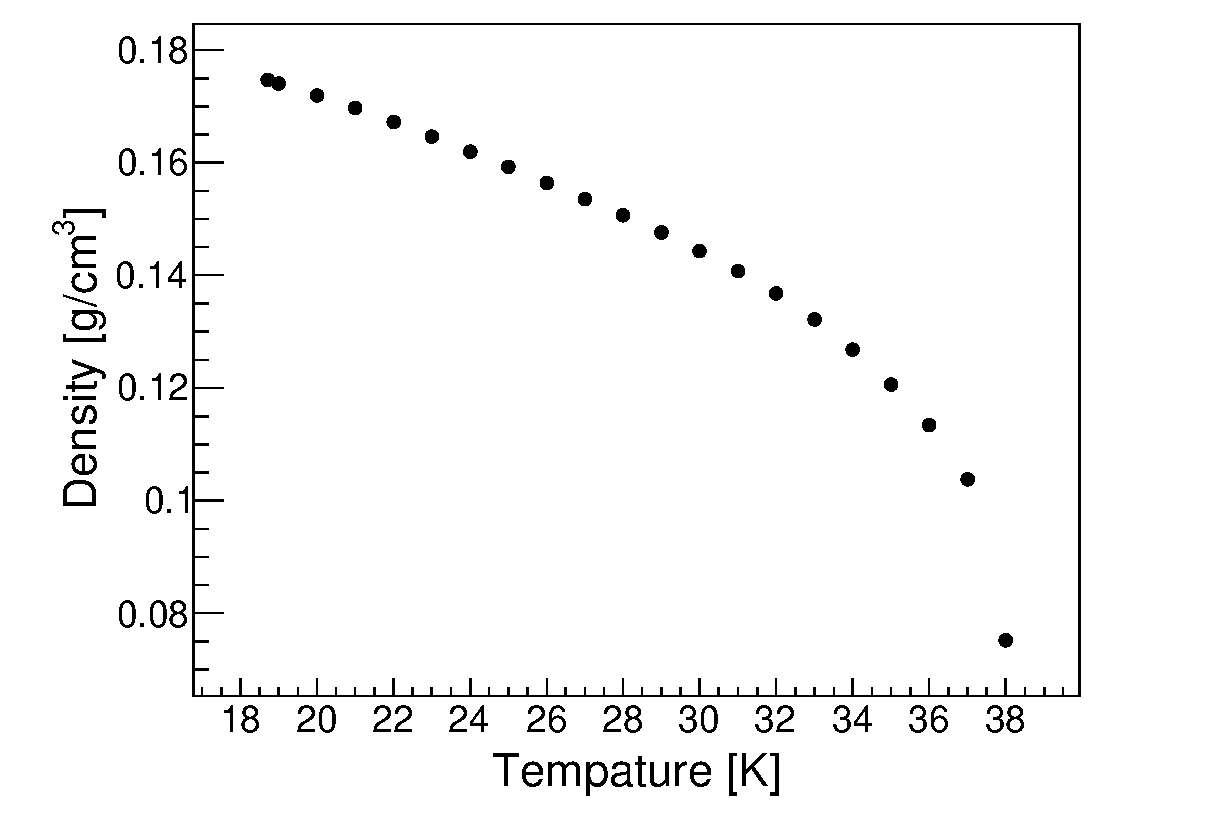
\includegraphics[width=5cm]{../pic/Dron/target/target_den.eps}
    \end{minipage}
  \end{tabular}
  \caption{
    The left figure shows the temperature of the $D_2$ target.
    The right figure shows the relation of the density and the $D_2$ temperature at 1 atm.
  }
  \label{fig:target}
\end{figure}


The target cell is $6.8cm$ diameter and $12.5cm$ length cylinder made of PET.
Liquifregrated $D_2$ is transferred by downpipe and warmed liquid $D_2$ by the heat load is returned through the upper pipe,
so the heat is effectively transferred between the target cell and the heat exchanger\cite{Target}.
Since the temperature range of liquid $D_2$ is narrow as 18.7-23.8K at 1 atm, the temperature of the $D_2$ should be controlled in the liquid range to avoid blocking due to the solid $D_2$.
Since the cooling power of the second stage of the G–M refrigerator is larger than the heat load on the low-temperature parts,
The current in the heater is controlled by a proportional-integral-derivative (PID) algorithm with an input of the temperature of the heat exchanger.
Target cell temperature in MR-RUN78 is represented in Fig\ref{fig:target} which is monitored by Pt-Co thermometer (CHINO R800-6) whose tolerance was $\pm$ 0.5K.
The same figure also shows the relation of temperature and density of $D_2$ at 1 bar.
The error of $D_2$ density was estimated at 1.5$\times 10^{-3} [g/cm^3]$ from tolerance and fluctuation.


%% \begin{frame}{CDC fine turning}
  \begin{tabular}{cc}
    \begin{minipage}{0.5\hsize}
      \begin{figure}
        Before\\
        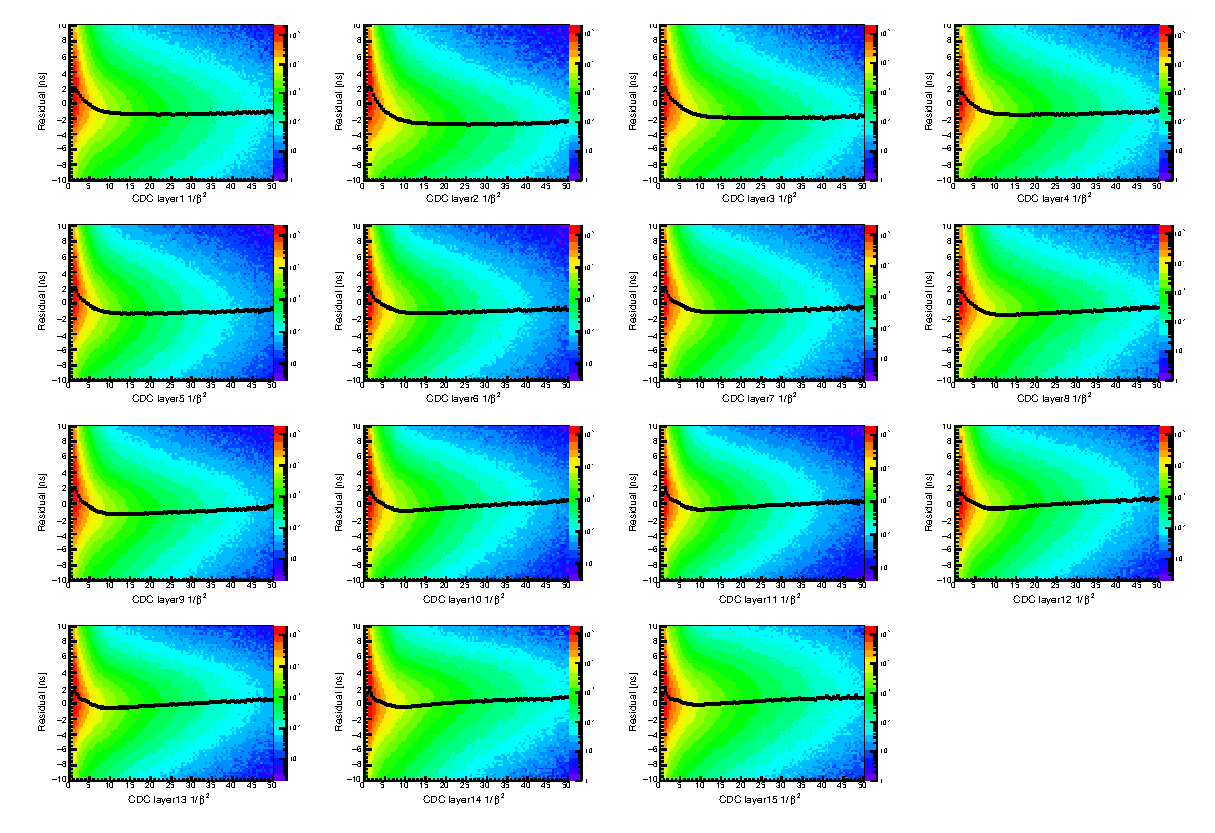
\includegraphics[width=5cm]{../pic/Run78/CDS/CDC_ob2_res_before.eps}
      \end{figure}
    \end{minipage}

    \begin{minipage}{0.5\hsize}
      \begin{figure}
        After\\
        \includegraphics[width=5cm]{../pic/Run78/CDS/CDC_ob2_res.eps}
      \end{figure}
    \end{minipage}
  \end{tabular}
  \centering
  $\beta$ and residual has correlation, which was calibrated wire-by-wire.
\end{frame}

\begin{frame}{Vertex image by CDS and BPC}
  \begin{figure}
    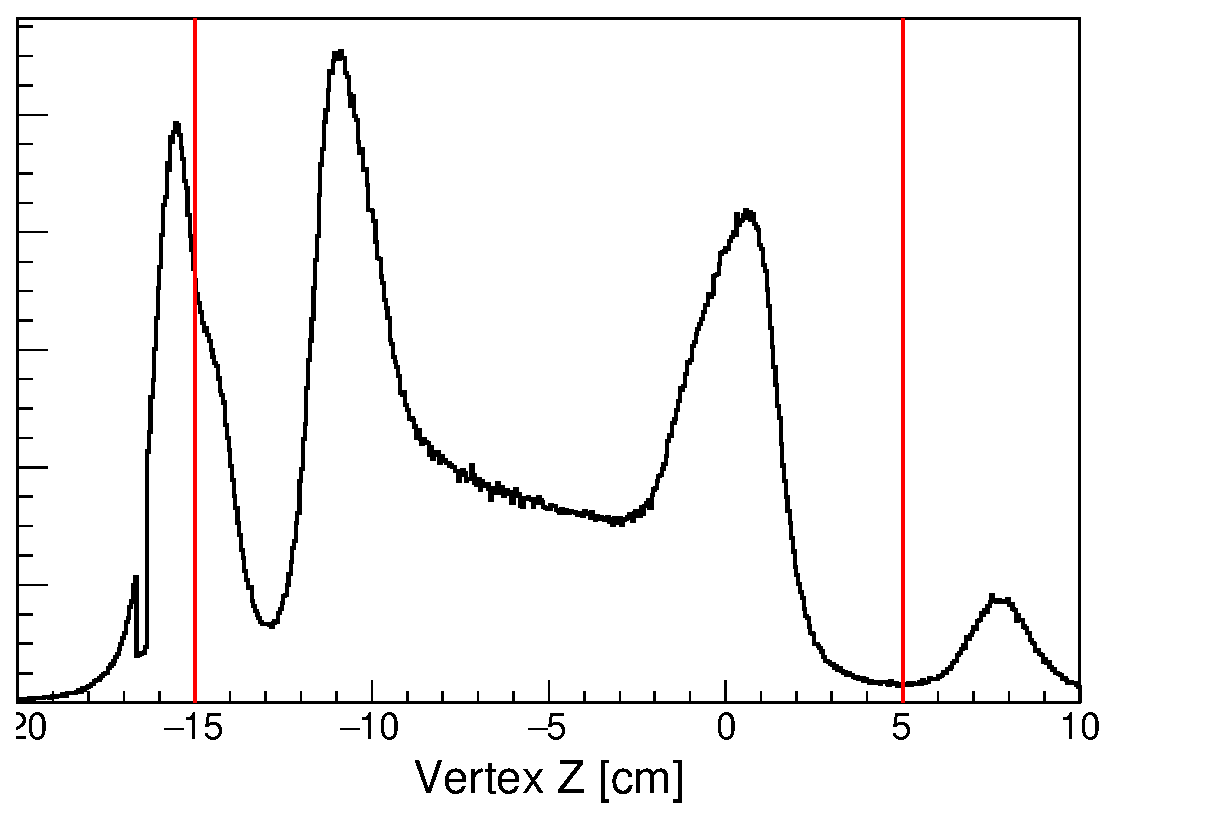
\includegraphics[width=8cm]{../pic/Run78/CDS/vertex.eps}
  \end{figure}
\end{frame}

\begin{frame}{Vertex image by CDS and BPC (Vertex cut)}
  \begin{figure}
    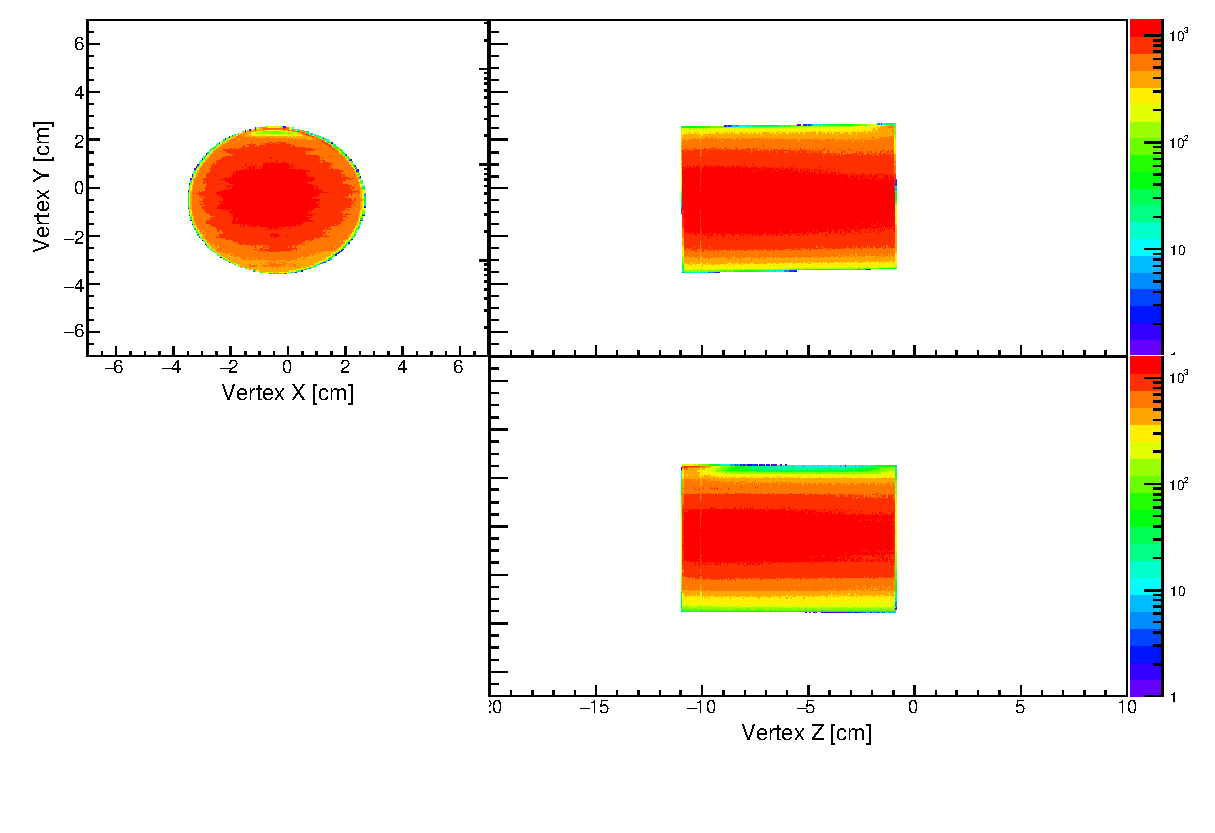
\includegraphics[width=8cm]{../pic/Run78/CDS/vertex_f.eps}
  \end{figure}
\end{frame}

\begin{frame}{Vertex resolution}
  \begin{tabular}{cc}
    \begin{minipage}{0.5\hsize}
      \begin{figure}
        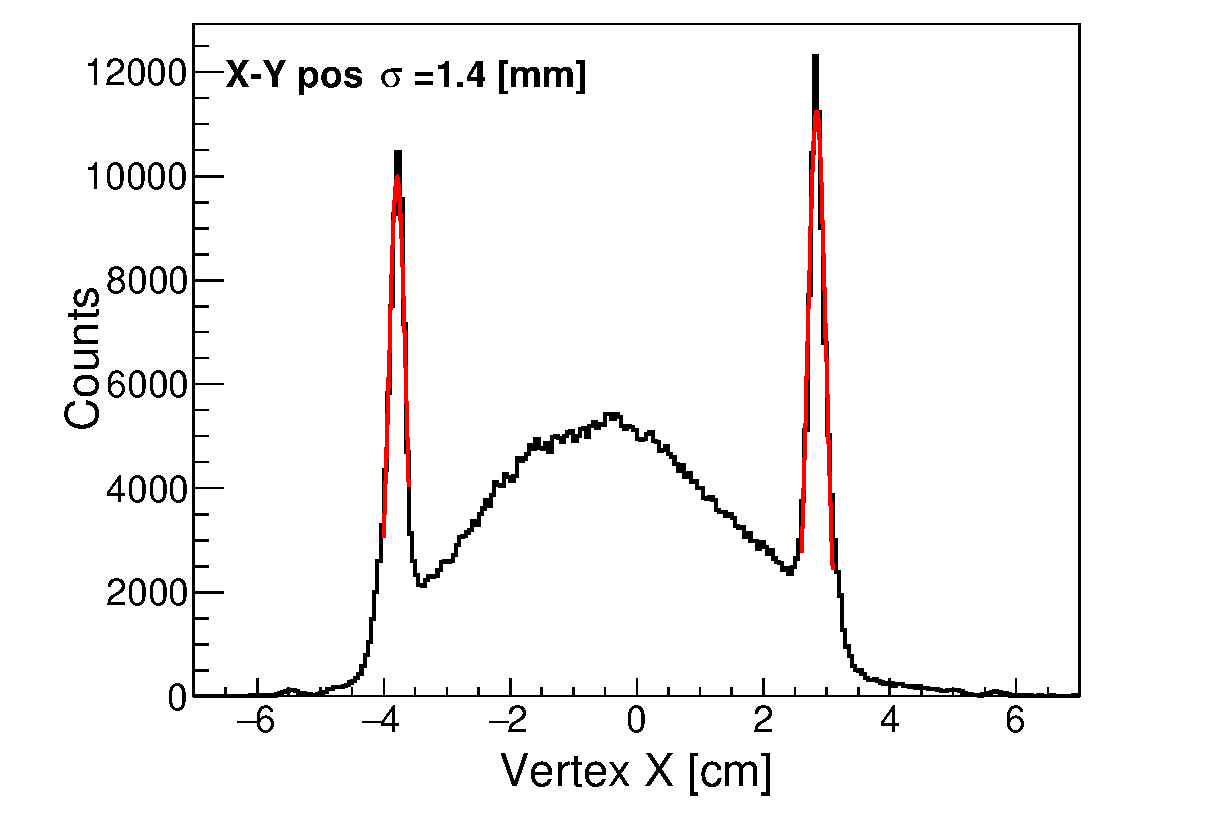
\includegraphics[width=5cm]{../pic/Run78/CDS/vertex_x.eps}
      \end{figure}
      \centering
      Y range was selected \\ $-5.5\sim-5$ [mm]
    \end{minipage}

    \begin{minipage}{0.5\hsize}
      \begin{figure}
        \includegraphics[width=5cm]{../pic/Run78/CDS/vertex_z.eps}
      \end{figure}
      \centering
      $Z =0$ was selected [mm]\\
      resolution was evaluated by DEF.
    \end{minipage}
  \end{tabular}
\end{frame}

\begin{frame}{CDS mass$^2$ vs momentum}
  \begin{figure}
    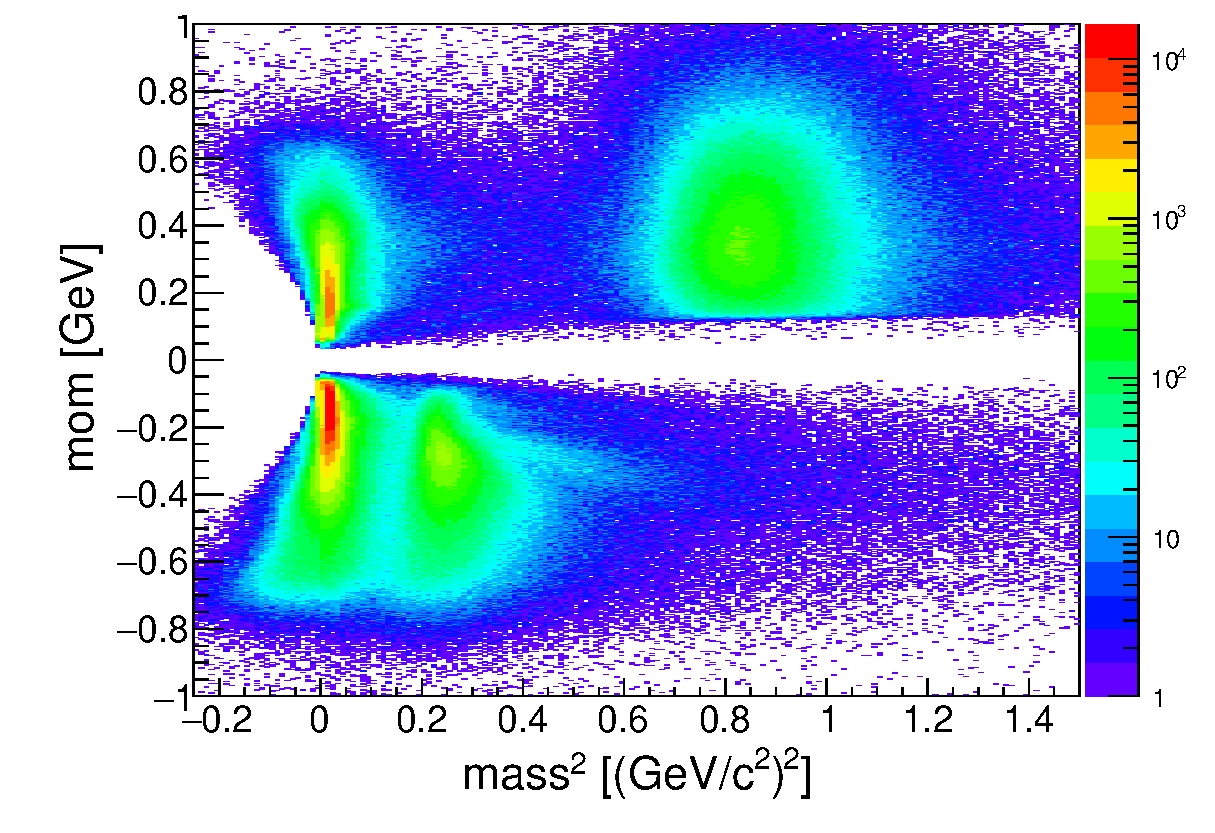
\includegraphics[width=8cm]{../pic/Run78/CDS/pid.eps}
  \end{figure}
\end{frame}

\begin{frame}{Invaraint mass by CDS}
  \begin{tabular}{cc}
    \begin{minipage}{0.5\hsize}
      \begin{figure}
        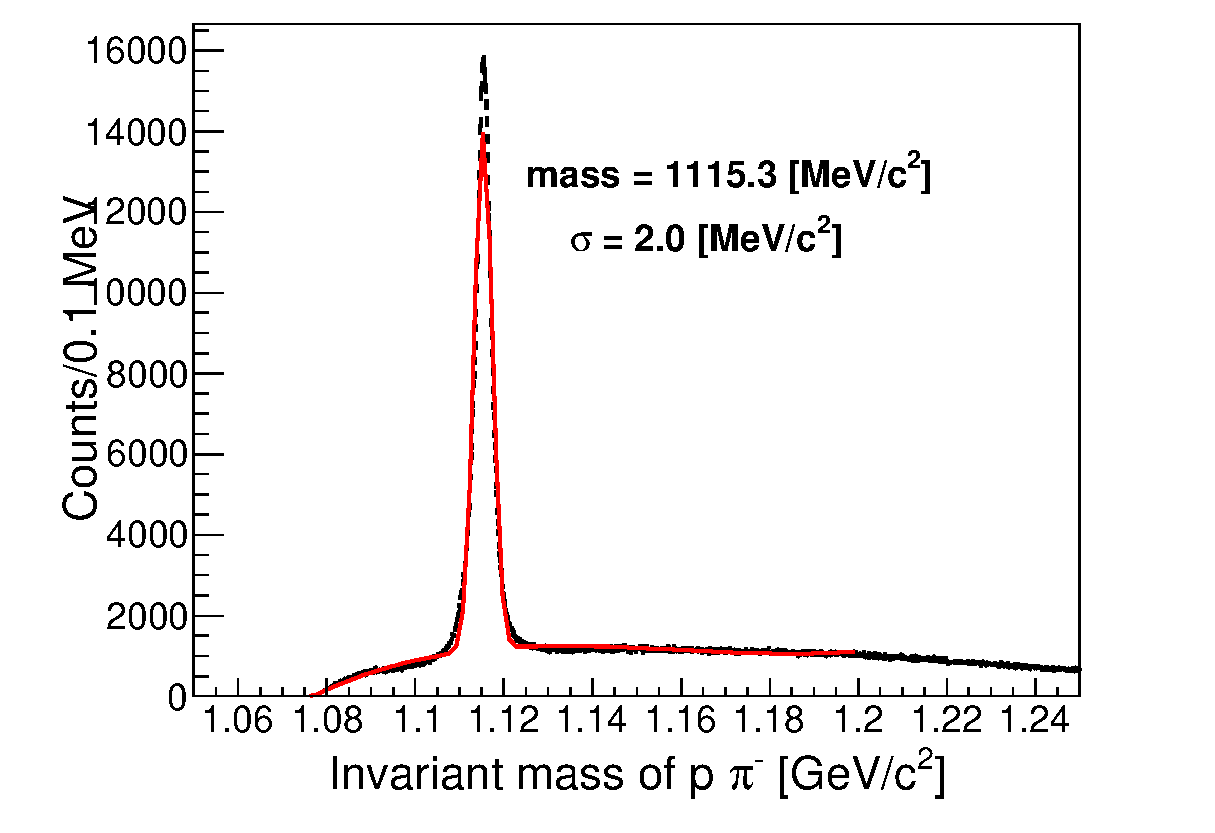
\includegraphics[width=5cm]{../pic/Run78/CDS/IM_ppim.eps}
      \end{figure}
    \end{minipage}

    \begin{minipage}{0.5\hsize}
      \begin{figure}
        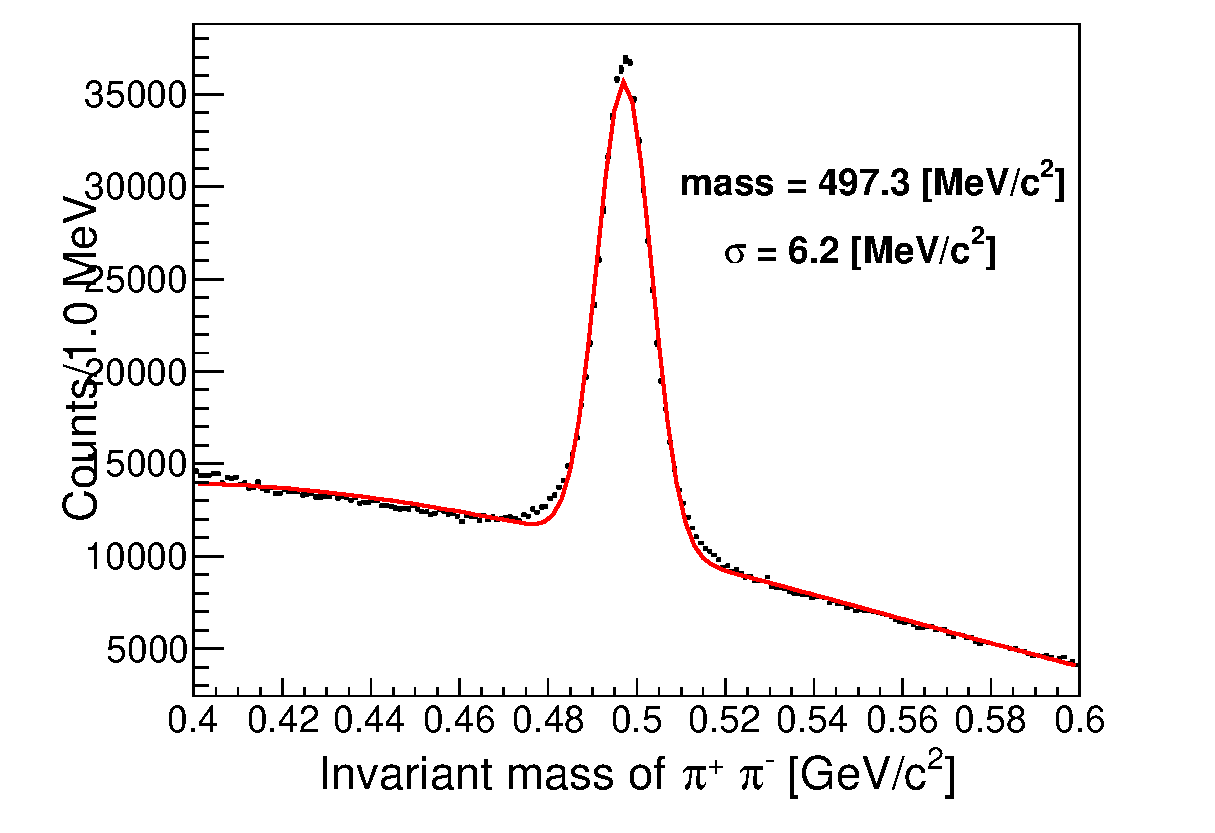
\includegraphics[width=5cm]{../pic/Run78/CDS/IM_pipi.eps}
      \end{figure}
    \end{minipage}
  \end{tabular}
\end{frame}




%% \section{Forward Detector System}
The forward detector system consists of a neutron detector system for detecting forward scattered neutrons
and a proton detector system for detecting protons, although some detectors are used for both purposes.

Downstream of the CDS is a beam sweep magnet, called Ushiwaka, which bends the negatively charged beam into a beam dump.
Positively charged particles are bent to the opposite side by the Ushiwaka, while neutrals fly straight.
The neutron counter (NC) is installed about 15 m downstream of the CDS to detect the neutral particles,
and the charge veto counter (CVC) is installed immediately upstream to confirm that they are not actually charged particles.

The Proton counter (PC) is installed in the opposite direction to the beam dump to detect positive charged particles.
The forward drift chamber (FDC) is installed upstream of the Ushiwaka to detect the position of positive charged particles before they are bent,
whose information is used to momentum analysis and particle identification.

The beam veto counter (BVC) is also installed immediately upstream of the FDC to detect beams that have passed through without reacting with the target, which is described.

\subsection{Beam Sweeping Magnet}
The beam sweep magnets, called Ushiwaka, are located 150 cm downstream of the target and have a pole length of 70 cm.
The aperture of the Ushiwaka is 82cm (horizontal) $\times$ 40cm (vertical), which is wider than the area covered by the NC in the present experimental setup.
The Ushiwaka can be applied to 1.6T at maximum value and is applied to 1.2T in the present experiment.


\subsection{Neutron Counter - NC}
The neutron counter (NC) are located 14.7 m upstream of the target.
Because the NC are located at the most upstream and the purpose is to detecting neutral particles, the NC requires a large amount of material.
Therefore, the NC is a segmented scintillation detector with 7 layers, each layer consisting of 16 counters.
One scintillation detector is 20cm (width) $\times$ 150cm (height) $\times$ 5cm (thickness) in size.
So one layer covers 320cm (width) $\times$ 150cm (height), which is corresponds 6.2 degrees in horizontal and 2.9 degrees in vertical in this experiment setup.
The first three layers of the scintillator are made of Saint-Gobain BC408 and the other four layers are made of Saint-Gobain BC412.
The scintillation light is carried by lucite light guides on both sides and read out by the 2-inch PMT (Hamamatsu H6410).
Each layer is installed with a gap of 2 cm, so the whole NC has a thickness of 47 cm.
Differences between the upstream and downstream solid angles are evaluated as systematic errors.

\subsection{Charge Veto Counter - CVC}
The charge veto counter (CVC) is installed just upstream of the NC to confirm that particles detected by the NC is actually neutral.
Half of the CVC is used to detect the proton.
The CVC consists of 34 segmented plastic scintillators whose size is 10cm (width) $\times$ 150cm (height) $\times$ 5cm (thickness).
A 2-inch Hamamatsu Photomultipliyer H6410 is attached to each side of the scintillator through a Lucite light guide.
The scintillator is of Eljen EJ-200 type. The average time resolution measured with cosmic rays is 78 $\pm$ 7 ps ($\sigma$).
The error represents the variation among the segments.

\subsection{Proton Counter - PC}
The proton detector (PC) is a hodoscope array for detecting positive charged particles located immediately next to the CVC in the direction opposite to the beam dump.
The PC is a 27-segmented detector using scintillators of the same size as the CVC, i.e. it has an effective area of 270 m (horizontal) $\times$ 150 m (vertical).
% However, charged particles are bent and their bending angle depends on their momentum, so their acceptance depends on their momentum.
The photomultipliyer of the PC is the same as the CVC, but the scintillator is a Saint-Gobian BC408.
The average time resolution measured with cosmic rays is 75 $\pm$ 6 ps ($\sigma$),  i.e. the time resolution does not differ from the CVC


\subsection{Forward Drift Chamber - FDC}
\begin{table}
  \caption{Summary of the beam-line chamber parameters.}
  \centering
  \begin{tabular}{l|cccc}
    \hline\hline
    &       BLC1a   &       BLC1b   &       BLC2a   &       BLC2b  \\
    \hline
    number of planes        &       8       &       8       &       8       &       8      \\
    plane configuration     &       \footnotesize{UU'VV'UU'VV'}     &       \footnotesize{UU'VV'UU'VV'}     &       \footnotesize{UU'VV'UU'VV'}     &       \footnotesize{VV'UU'VV'UU'} \\
    \shortstack{number of sense wires \\ in a plane}        &       32      &       32      &       32      &       32     \\
    wire spacing (mm)       &       4       &       4       &       2.5     &       2.5     \\
    effective area (mm)     &       256 $\times$ 256        &       256 $\times$ 256        &       160 $\times$ 160        &       160 $\times$ 160       \\
    \hline
    Sense wire              &               &               &                               &     \\
    ~~material              &       \multicolumn{4}{c}{Au-plated W (3\% Re)}                     \\
    ~~diameter ($\mu m$)    &       \multicolumn{4}{c}{ 12}                                      \\
    \hline
    Potential wire          &               &               &                               &     \\ 
    ~~material              &       \multicolumn{4}{c}{Au-plated Cu-Be}                          \\
    ~~diameter ($\mu m$)    &       \multicolumn{4}{c}{ 75}                                      \\
    \hline
    Cathode plane           &              &                &               &   \\
    ~~material              &       \multicolumn{4}{c}{alminized-Kapton}       \\
    ~~thickness ($\mu m$)   &       \multicolumn{4}{c}{12.5}                   \\
    %% \hline
    %% Gas             &       \multicolumn{4}{c}{ Ar : isoC$_4$H$_{10}$ : Metylal = 76 : 20 :4}   \\
    %% flow (cc/min)   &       \multicolumn{4}{c}{100}                                             \\
    %%    %% %plane efficiency       &       $>$ 99\%        &       $>$ 99\%        &       $>$ 99\%        &       $>$ 99\%        &       $>$ 99\%        &       $>$ 99\%        \
    \hline\hline
    operation voltage       &               &               &               &               \\
    potential               &       -1.25   &       -1.25   &       -1.25   &       -1.25   \\
    cathord                 &       -1.25   &       -1.25   &       -1.25   &       -1.25   \\
    %guard  &       -       &       -       &       -       &       -       &       -       &       -1.85   \\
    \hline\hline
  \end{tabular}

  \begin{tabular}{l|ccc}
    \hline\hline
    &       BPC(Run68)   &  BPC(Run78)   &  FDC1 \\
    \hline
    number of planes        &       8       &       8       &       6     \\
    plane configuration     &       \footnotesize{XX'YY'X'XY'Y}     &       \footnotesize{XX'YY'X'XY'Y}     &       \footnotesize{UU'XX'VV'}  \\
    \shortstack{number of sense wires \\ in a plane}        &       15      &       32      &       64      \\
    wire spacing (mm)       &       3.6       &       3       &     3           \\
    effective area (mm)     &       111.6$\phi$       &  189$\phi$        &      \\
    \hline
    Sense wire              &               &                                &            \\
    ~~material              &       \multicolumn{3}{c}{Au-plated W (3\% Re)}                   \\
    ~~diameter ($\mu m$)    &       \multicolumn{2}{c}{ 12}                  &      12   \\
    \hline
    Potential wire          &                            &               &               \\ 
    ~~material              &       \multicolumn{2}{c}{Au-plated Cu-Be}  &  Au-plated Cu-Be \\
    ~~diameter ($\mu m$)    &       \multicolumn{2}{c}{ 75}              &   75      \\
    \hline
    Cathode plane           &                    &                &             \\
    ~~material              &       \multicolumn{2}{c}{Cu aramid} & alminaized-Kapton \\
    ~~thickness ($\mu m$)   &       \multicolumn{2}{c}{9}         & 7.5     \\
    %% \hline
    %% Gas             &       \multicolumn{4}{c}{ Ar : isoC$_4$H$_{10}$ : Metylal = 76 : 20 :4}   \\
    %% flow (cc/min)   &       \multicolumn{4}{c}{100}                                             \\
    %% %% %plane efficiency       &       $>$ 99\%        &       $>$ 99\%        &       $>$ 99\%        &       $>$ 99\%        &       $>$ 99\%        &       $>$ 99\%        \
    \hline\hline
    operation voltage       &               &               &                      \\
    potential               &       -1.50   &       -1.45   &       -1.45          \\
    cathord                 &       -1.50   &       -1.45   &       -1.45          \\
    %guard  &       -       &       -       &       -       &       -       &       -       &       -1.85   \\
    \hline\hline
  \end{tabular}

  \label{tab:chamber}
\end{table}

For forward scattered positive particles,
The forward drift chamber (FDC) is installed immediately upstream of the Ushiwaka to measure the trajectory of the charged particles before they are bent for momentum analysis.
The information is used for momentum analysis of forward-scattered positive particles for particle identification.

Each pairs are separated by a 20 mm gap using aluminised-Kapton.
The sense wires are arranged with a 6 mm gap and the electric field is created by potential wires surrounding them with squares.
The sense wires and potential wires are the same wires used in the BLC and the BPC.
% The FDC1 has a 400mm (horizontal) $times$ 300mm (vertival) open window, so its effective erea is 363mm (horizontal) $times$ 300mm (vertical) when evaluated as a rectangle.
The configuration of the BLC1/2 and the BPC and the FDC is summarized in Table.\ref{tab:chamber}.
These drift chambers is used same gas.

\subsection{Beam Veto Counter - BVC}
\subsection{Beam Veto Counter - BVC}
\input{experimental/figs/BVC}
The BVC is installed immediately upstream of the FDC to avoid beams that did not react with the target.
Its signal is mainly used for forward neutron triggering.
The BVC are installed as horizontal counters with various width due to the vertical dependence of the particle density.
The coverage size of the BVC is 320mm (height) $\times$ 320mm (width) with 10 (thickness) of scintillators, as shwon in Table.\ref{fig:BVC}.
The scintillator is used ELJEN EJ-200.


The BVC is installed immediately upstream of the FDC to avoid beams that did not react with the target.
Its signal is mainly used for forward neutron triggering.
The BVC are installed as horizontal counters with various width due to the vertical dependence of the particle density.
The coverage size of the BVC is 320mm (height) $\times$ 320mm (width) with 10 (thickness) of scintillators, as shwon in Table.\ref{fig:BVC}.
The scintillator is used ELJEN EJ-200.




%% \begin{frame}{DAQ efficeincy}
  \begin{figure}
    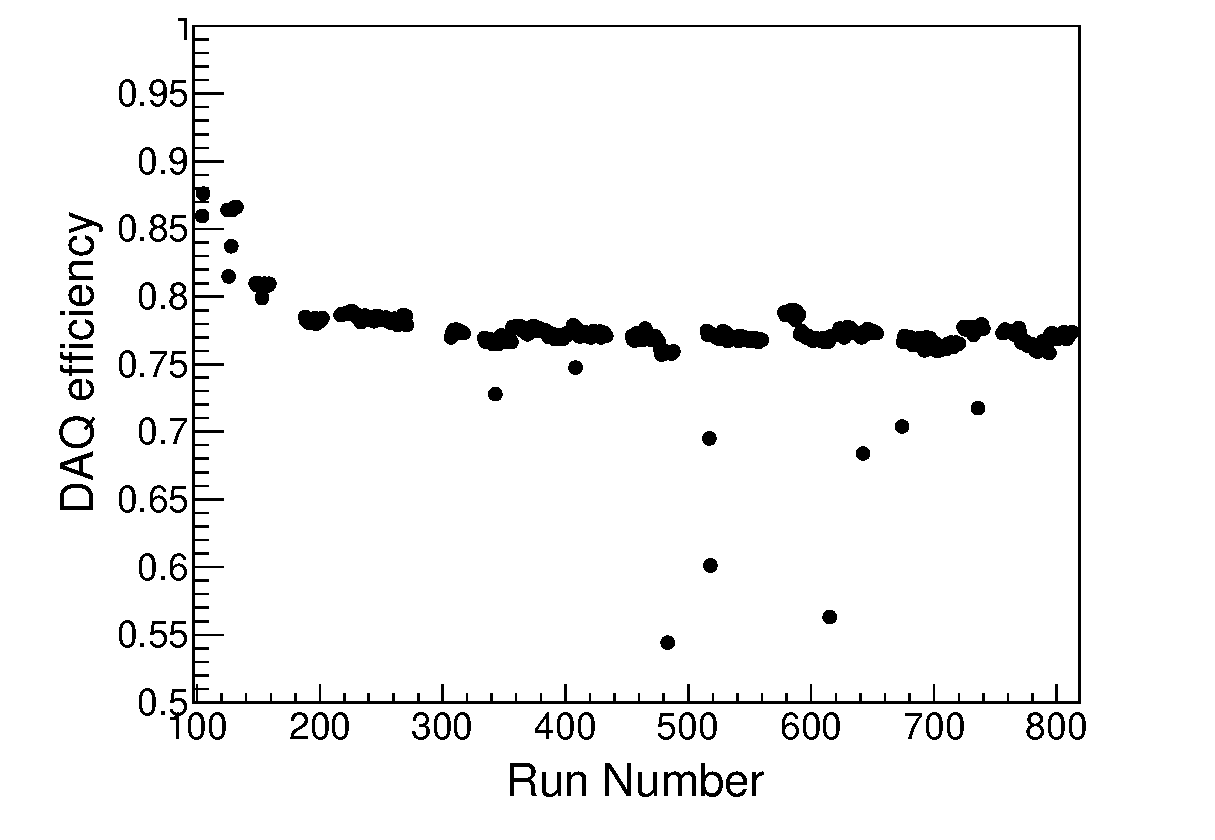
\includegraphics[width=8cm]{../pic/Run78/trigger/DAQ.eps}
  \end{figure}
\end{frame}

